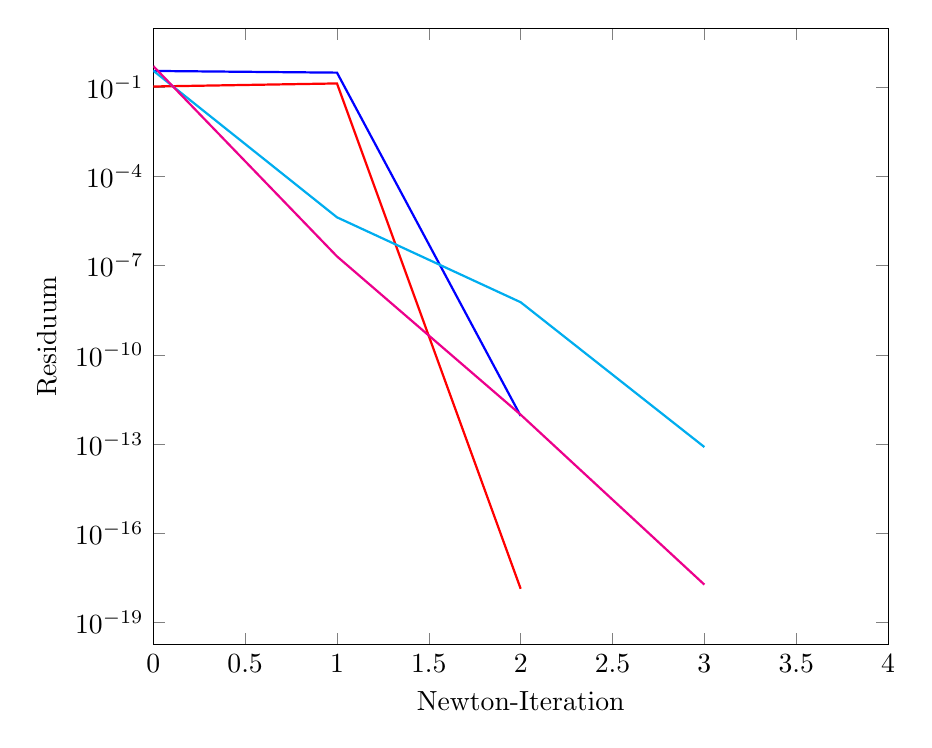
\begin{tikzpicture}[every plot/.append style={thick}] 
\begin{axis}[ 
label style={font=\normalsize}, 
xlabel={Newton-Iteration}, 
ylabel={Residuum}, 
xmin=0, xmax=4, 
ymode=log, 
ymin=0, ymax=10, 
width=0.9\textwidth, 
grid style=dashed, 
] 
\addplot[ 
color=blue, 
] 
coordinates { 
(0, 3.64e-01)(1, 3.19e-01)(2, 8.70e-13)}; 
\addplot[ 
color=red, 
] 
coordinates { 
(0, 1.09e-01)(1, 1.38e-01)(2, 1.31e-18)}; 
\addplot[ 
color=cyan, 
] 
coordinates { 
(0, 3.70e-01)(1, 4.27e-06)(2, 5.88e-09)(3, 7.80e-14)}; 
\addplot[ 
color=magenta, 
] 
coordinates { 
(0, 5.30e-01)(1, 2.06e-07)(2, 9.59e-13)(3, 1.81e-18)}; 
\end{axis} 
\end{tikzpicture} 
